\section{The \sys System}
\label{sec:pithtrain}


\subsection{Agent-Native Design Principles}
\label{sec:pithtrain:principles}

This subsection introduces the four agent-native design principles
that guide \sys's system design, and contrasts how production
training frameworks align with each principle today.
\autoref{tab:principles-comparison} summarizes this comparison;
production frameworks adopt different subsets of the four
principles, reflecting different design priorities.

\begin{table}[t]
  \centering
  \small
  \caption{Adherence to agent-native design principles.
  \cmark{} satisfied; \pmark{} partial; \xmark{} not satisfied.
  Numbers are total framework LoC across Python, C++, and CUDA.\protect\footnotemark}
  \label{tab:principles-comparison}
  \begin{tabular}{lcccc}
    \toprule
    Framework & Compact & Python-native & No implicit indirection & Agent skills \\
    \midrule
    \megatron    & \xmark~149K  & \xmark & \xmark & \pmark \\
    \deepspeed   & \xmark~167K  & \xmark & \xmark & \xmark \\
    \torchtitan  & \pmark~38K   & \cmark & \pmark & \pmark \\
    \textbf{\sys} & \cmark~11K & \cmark & \cmark & \cmark \\
    \bottomrule
  \end{tabular}
\end{table}
\footnotetext{LoC measured at the pinned commits \texttt{3bec9aa}
(\megatron), \texttt{44c51e3} (\deepspeed), \texttt{d84e83d}
(\torchtitan), and \sys at v0.1.2.}


\MyPara{Compact codebase.}
Production frameworks such as \megatron and \deepspeed offer broad
coverage of models, training features, and hardware platforms,
accumulated over years of engineering effort, with core codebases
exceeding 160K lines. A larger codebase inflates the cost of
locating relevant code, tracking cross-file dependencies, and
verifying a change is complete. A compact codebase reduces this
cost; with frontier coding agents operating at context windows of
200K to 1M tokens, a sufficiently compact codebase can also fit in
a single context pass. We treat compactness as a constraint on
growth: \sys may grow over time, but additions should respect
the four principles.

\MyPara{Python-native codebase.}
Python is the dominant language in modern ML.
A pure-Python framework lets an agent navigate the full framework
in a single language, surfaces readable Python tracebacks instead
of opaque native errors, and eliminates the compiled-extension
rebuild cycle. \megatron composes its core transformer layers from
out-of-tree TransformerEngine~\cite{transformer-engine} modules,
and \deepspeed bundles extensive in-tree extensions. These deliver
peak kernel performance and vendor-tuned numerics, but push an
agent across language boundaries and force a rebuild on change.

\begin{figure}[t]
  \centering
  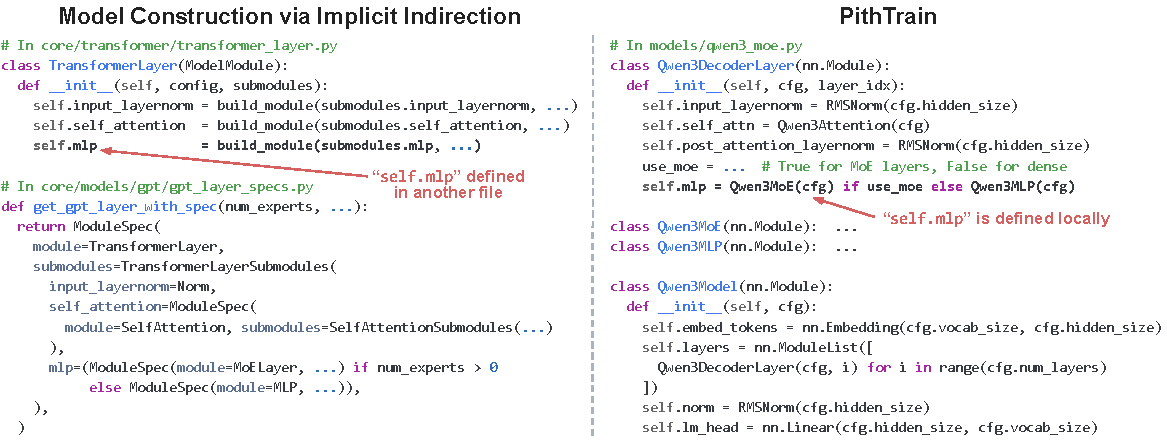
\includegraphics[width=0.9\textwidth]{figures/fig2_implicit_indirection.pdf}
\caption{Model construction patterns, illustrating the
  no-implicit-indirection principle. The implicit-indirection pattern
  resolves submodules through a runtime spec, supporting model
  variation from a shared layer skeleton; \sys instantiates
  layers directly, favoring local readability.}
  \label{fig:indirection-contrast}
\end{figure}

\MyPara{No implicit indirection.}
Production frameworks compose many model variants from a shared
layer skeleton via \emph{implicit indirection} (a stored
callable, plugin registry, or string-keyed resolution). This
pattern enables code reuse across models, while making what runs
at a given call site harder to identify by local reading.
\autoref{fig:indirection-contrast} shows an instance of model
construction in a production framework: \texttt{TransformerLayer}
resolves its submodules from a runtime spec in a separate file.
A flat code structure trades cross-model reuse for local
readability, reducing the effort an agent spends building an
end-to-end understanding.

\MyPara{Task-specific agent skills.}
An \emph{agent skill}~\cite{anthropic-skills} is a procedural
playbook a coding agent loads on demand. Skills encode procedural knowledge an agent cannot recover from static reading alone, so it
runs a verified procedure. Agent
skills are a recent practice that existing training frameworks
have not yet adopted at scale: \megatron ships six skills for
CI/PR hygiene; \torchtitan ships one
developer-workflow skill plus four editor rules orienting the
agent to the codebase; \deepspeed ships two markdown files with
generic rules. None of these target recurring training-framework
tasks.


\subsection{System Architecture and Optimizations}
\label{sec:pithtrain:arch-and-opt}

\begin{figure}[t]
\centering
\begin{minipage}[c]{0.58\textwidth}
  \centering
  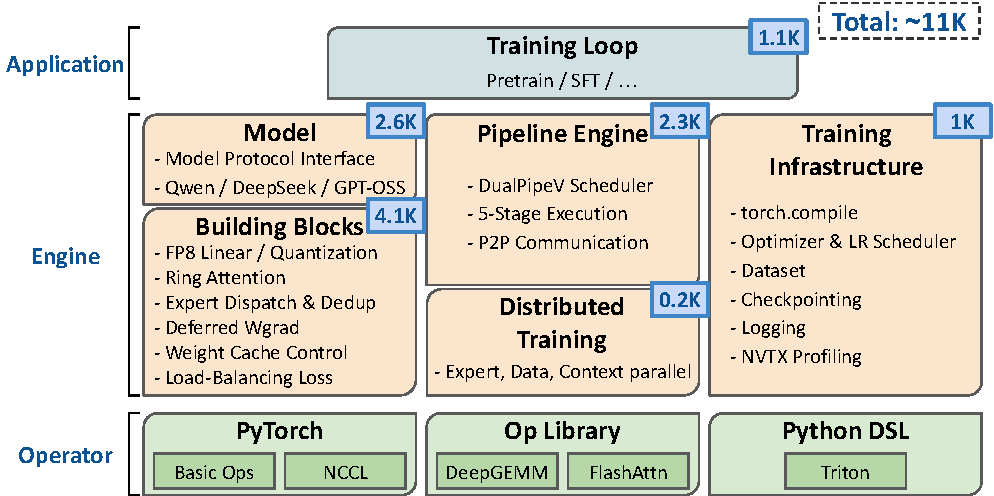
\includegraphics[width=\textwidth]{figures/fig3_architecture.pdf}
  \caption{\sys architecture with per-component line counts.}
  \label{fig:arch}
\end{minipage}%
\hfill
\begin{minipage}[c]{0.40\textwidth}
  \captionof{table}{Where \sys realizes each principle.}
  \label{tab:principle-map}
  \vspace{2pt}
  {\small
  \begin{tabular}{@{}>{\raggedright\arraybackslash}p{0.40\linewidth}@{\hspace{2pt}}>{\raggedright\arraybackslash}p{0.59\linewidth}@{}}
    \toprule
    Principle & Where it lives \\
    \midrule
    Compact codebase & All boxes in \autoref{fig:arch}; line counts sum to $\sim$11K \\
    \addlinespace
    Python-native codebase & Whole stack; Python-DSL for custom kernels only \\
    \addlinespace
    No implicit indirection & Whole codebase; flat structure \\
    \addlinespace
    Agent skills & Specialized skills under the project root \\
    \bottomrule
  \end{tabular}%
  }
\end{minipage}
\end{figure}

The codebase is organized in three layers (application, engine, operator), as shown in \autoref{fig:arch}.
To realize a compact codebase, we identified the necessary
components for a distributed MoE training framework, and \sys covers
exactly those. Where production
frameworks deliver broad out-of-the-box coverage of models,
features, and hardware, \sys narrows scope to keep the codebase
compact and reachable in a single context window.
Table~\ref{tab:principle-map} maps each principle to where it is
realized: we adopt a flat code structure with no plugin registries
or runtime specs, with each MoE model living in a self-contained
file under \texttt{models/} rather than being composed through a
shared layer skeleton. This favors local readability over cross-model
code reuse.

\sys supports standard MoE training\footnote{\sys also supports
dense (non-MoE) models, with MoE-specific machinery (e.g., expert
parallelism) skipped.} with pipeline parallelism (PP),
data parallelism (DP) via FSDP~\cite{pytorchfsdp}, context
parallelism (CP)~\cite{liu2024ringattention}, expert parallelism
(EP)~\cite{lepikhin2020gshardscalinggiantmodels}, FP8
training~\cite{micikevicius2022fp8formatsdeeplearning}, and DCP
checkpointing~\cite{torch-dcp}, on NVIDIA Hopper and Blackwell GPUs.
Despite its compact, Python-native codebase, \sys aims for
training throughput competitive with production frameworks by
adopting standard MoE optimizations; these techniques are not novel, but they are
central to \sys's training throughput and worth calling out.

\squishlist
\item \textbf{DualPipeV pipeline schedule and compute--communication overlap.}
\sys's pipeline scheduler builds on DualPipe from
DeepSeek-V3~\cite{deepseekai2025deepseekv3technicalreport}. DeepSeek's
open-source version provides a minimal pipeline-orchestration
scaffold, on top of which \sys implements the actual
compute--communication overlap. Each transformer layer is
decomposed into five stages at EP communication boundaries. EP
all-to-alls run on a separate communication stream, and the schedule
overlaps the forward of one micro-batch with the backward of another.

\vspace{-2pt}

\item \textbf{Torch compile.}
\sys applies \texttt{torch.compile(fullgraph=True)} to all
transformer computation except the MoE forward and backward. This
strict mode rejects graph breaks at compile time rather than
silently degrading speedup. We exclude the MoE forward and
backward because per-expert input shapes are data-dependent under
expert parallelism.

\vspace{-2pt}

\item \textbf{Other optimizations.}
\sys also implements
wgrad delay~\cite{qi2024zero}; fused SwiGLU~\cite{shazeer2020gluvariantsimprovetransformer} forward and
backward kernels for throughput and reduced activation memory; EP
dispatch deduplication for lower all-to-all communication volume;
an FP8 weight cache across micro-batches to avoid re-quantization;
and fused Triton kernels for EP token scatter and FP8 quantization.
\squishend


\subsection{Agent Skills}
\label{sec:pithtrain:skills}

A skill encodes the procedure for one recurring training-framework
task. \sys ships a suite of skills covering several common ones
(Table~\ref{tab:skills}). Each skill is a self-contained folder with
a top-level \texttt{SKILL.md} playbook, optionally additional markdown
documents, and optionally helper scripts. Some skills are pure
markdown, like \texttt{add-new-model}; others bundle scripts that
offload deterministic work.

\begin{figure}[t]
\centering
\begin{minipage}[c]{0.48\textwidth}
  \captionof{table}{Representative skills in \sys.}
  \label{tab:skills}
  \vspace{2pt}
  {\small
  \begin{tabular}{@{}p{0.32\linewidth}@{\hspace{6pt}}>{\raggedright\arraybackslash}p{0.60\linewidth}@{}}
    \toprule
    Skill & Purpose \\
    \midrule
    \texttt{add-\allowbreak{}new-\allowbreak{}model} & Port a new MoE architecture end-to-end (model, FSDP, tests) \\
    \addlinespace
    \texttt{add-\allowbreak{}memory-\allowbreak{}prints} & Instrument training for memory profiling \\
    \addlinespace
    \texttt{capture-\allowbreak{}nsys-\allowbreak{}profile} & Capture an Nsight Systems profile of a short \sys run \\
    \addlinespace
    \texttt{validate-\allowbreak{}correctness} & Compare per-step loss curves between branches \\
    \bottomrule
  \end{tabular}%
  }
\end{minipage}%
\hfill
\begin{minipage}[c]{0.48\textwidth}
  \centering
  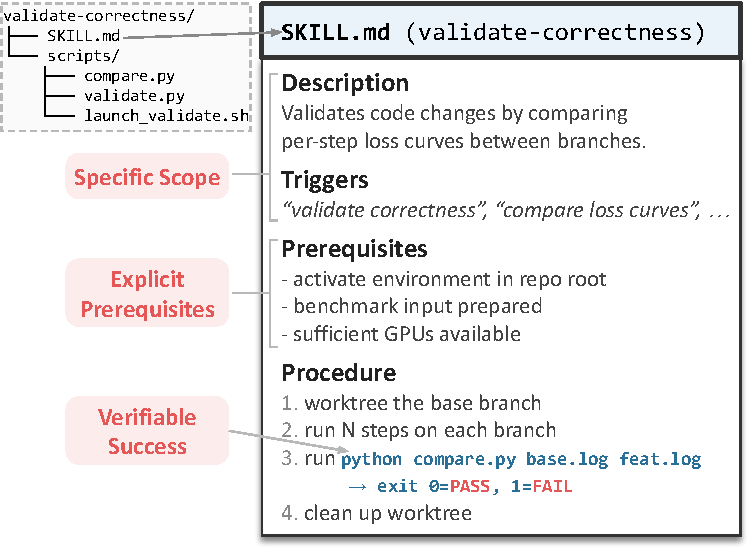
\includegraphics[width=0.95\textwidth]{figures/fig4_skill}
  \caption{The \texttt{validate-correctness} skill in \sys. Pink labels mark properties.}
  \label{fig:skill-anatomy}
\end{minipage}
\vspace{-10pt}
\end{figure}

Each skill in \sys is designed around three properties:
\emph{specific scope}, \emph{explicit prerequisites}, and
\emph{verifiable success}. \autoref{fig:skill-anatomy} illustrates
these on \texttt{validate-correctness}. The description and triggers
together encode the skill's specific scope. The prerequisites section
enumerates environment, data, and configuration assumptions, so
missing state is caught before the skill begins to run. The procedure
ends in a script call that returns a reproducible PASS/FAIL verdict
rather than the agent's self-assessment. Skills designed around these
properties are not technically hard to author, and we expect other
training frameworks to ship comparable coverage as the practice
matures.